\addcontentsline{toc}{chapter}{Messdaten} % damit trotzdem im Inhaltsverzeichnis
\label{Protokoll}


% \thispagestyle{empty}

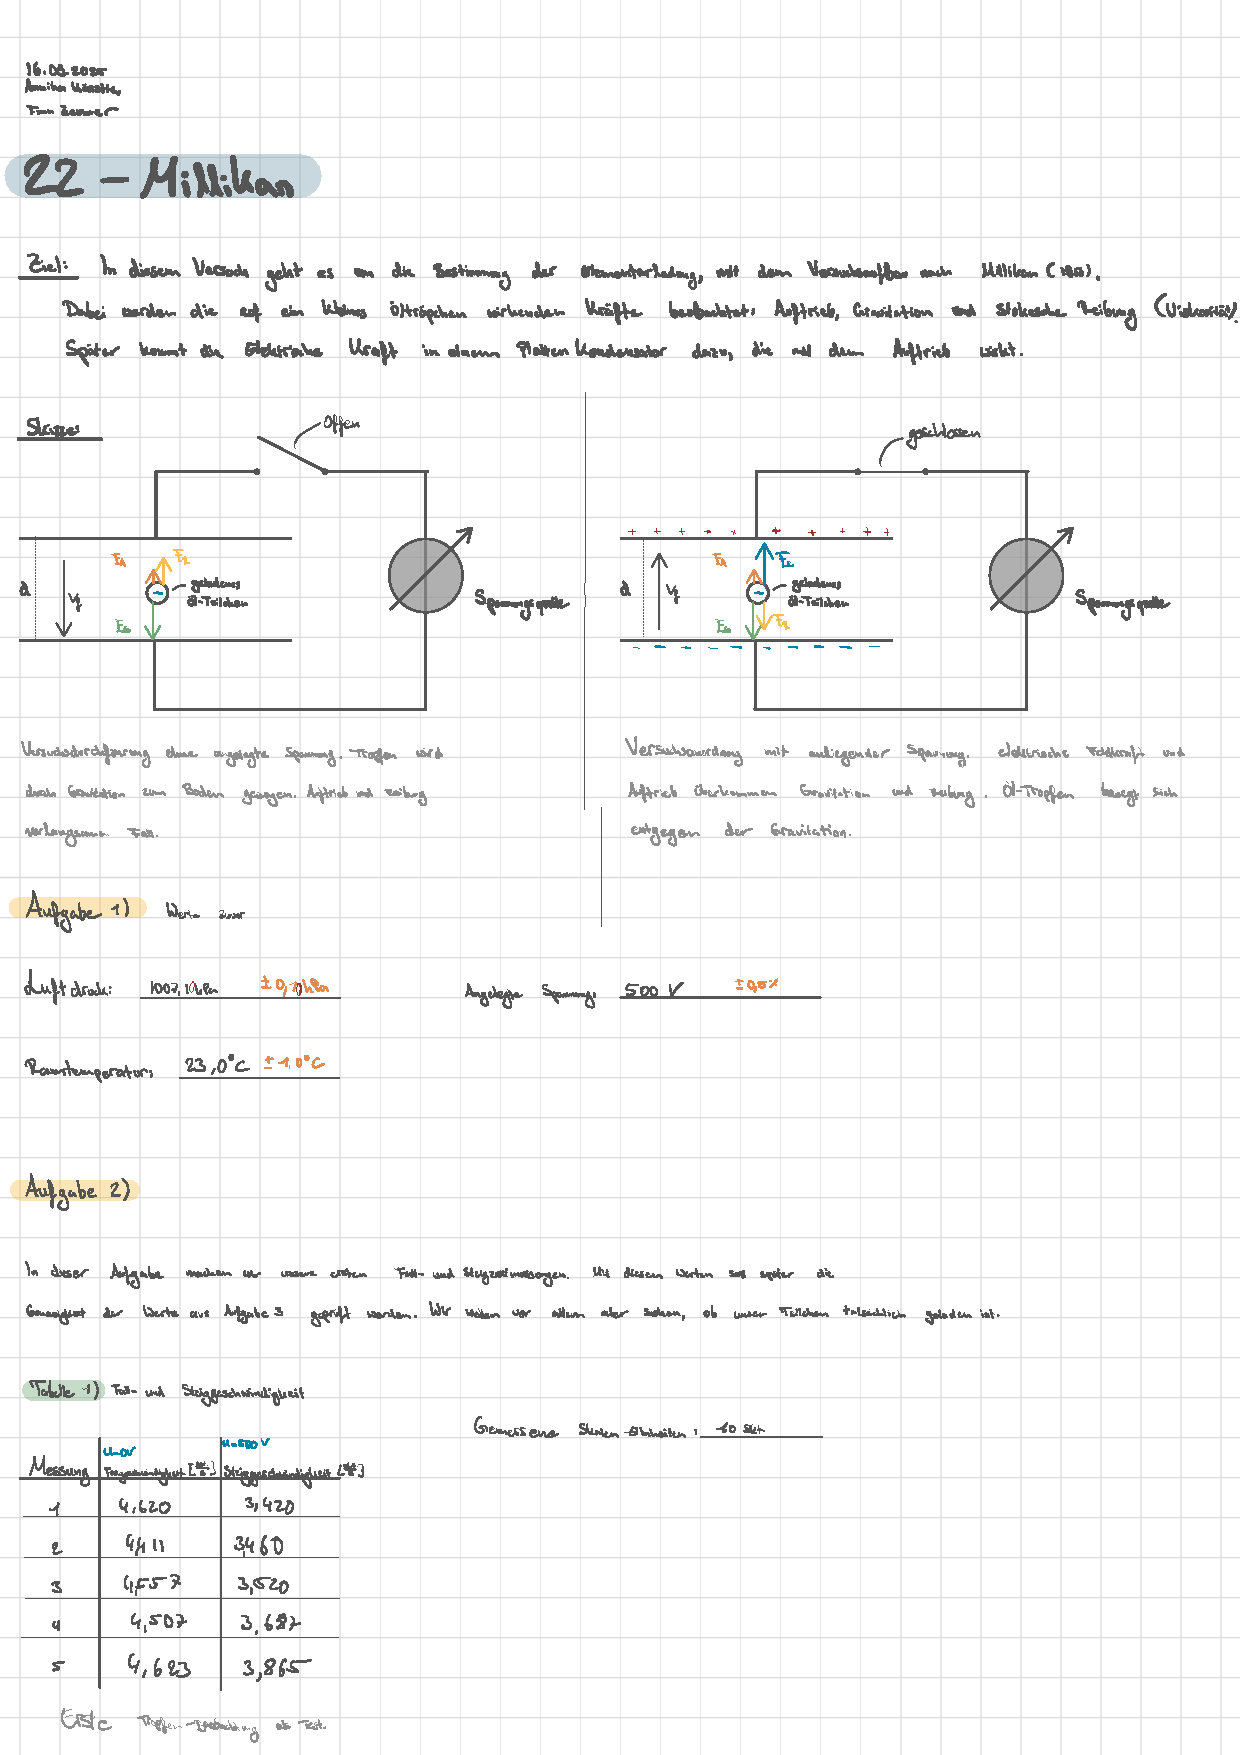
\includepdf[
  pages=1-3,               
  pagecommand={\thispagestyle{empty}} 
]{Protokolle/\versuchsnummer/Chapter/Messprotokoll.pdf}



\addcontentsline{lot}{table}{\protect\numberline{\thechapter.1} Gemessene Spannung mit mA-Meter}
\addcontentsline{lot}{table}{\protect\numberline{\thechapter.2} Gemessene Spannung mit Kompensator}
\addcontentsline{lot}{table}{\protect\numberline{\thechapter.3} Gemessener Strom am mA-meter und am Kompensator mit Schiebewiderstand}
